\documentclass{project-logbook}
\newcommand{\N}{\mathbb{N}}
\newcommand{\Z}{\mathbb{Z}}
\newcommand{\R}{\mathbb{R}}
\newcommand{\F}{\mathbb{F}}
\newcommand{\C}{\mathbb{C}}
\newcommand{\Q}{\mathbb{Q}}
\newcommand{\e}{\varepsilon}
\newcommand{\p}{\varphi}
\newcommand{\bfb}{\mathbf{b}}
\newcommand{\lr}[3]{\!\left#1 #3 \right#2} 
\newcommand{\lrbrace}[1]{\!\left\{ #1 \right\}} 
\newcommand{\imp}{\Longrightarrow}
\newcommand{\stline}{\;\middle\vert\;}
\newcommand{\floor}[1]{\left\lfloor#1\right\rfloor}
\newcommand{\ceil}[1]{\left\lceil#1\right\rceil}
\newcommand{\inv}{^{-1}}
% \newcommand{\norm}[1]{\left\lVert#1\right\rVert}
% \newcommand{\abs}[1]{\left\lvert#1\right\rvert}
\newcommand{\lrangle}[1]{\left\langle#1\right\rangle} % Inner product
\newcommand{\sub}{\leqslant}
\newcommand{\nsub}{\triangleleft}
\newcommand{\card}[1]{\overline{\overline{#1}}}

\usepackage{csquotes}
\usepackage{lastpage}
% You can add the maintainer and the contributors in the preamble of the document

% This is how you add the maintainer (there is only one) the maintainer is automatically a contributor, the format is
% name, id (to appear in short messages), the affiliation.
\SetMaintainer{Jeffrey Liang}{u7013004}{ANU School of Computing}

% This is how you add a contributor, you can have as many contributors as you like (althought
% there is a limited space on the front page, at least 25 contributors fit in the front page, which should
% be more than enought).
% The format is similar to Maintainer: key, name, id, affiliation. The key field is the difference. It is used
% to internally identify the contributor, such that one can access the data of each contributor. This is discussed
% below.


% The same goes for the titles of the project.
% Three levels can be used. The project title sets the main title of the project, which appears in the middle of the front page.
% The project subtitle appears below the project title in the front page and serves as additional information to the title.
%  Additionally, a shorter title must be set to appear on the header of the document, the header name.
\SetProjectTitle{Honours Logbook}
\SetProjectSubtitle{Semester 1 2024 - Semester 1 2025}
\SetProjectHeaderName{The very fancy project}

% Below the project there is space to add a brief summary of the project for easy understanding when looking at the front page.
\SetProjectSummary{This logbook contains notes and updates on my progress and findings throughout my Honours year.}

% The institution logo (typically the one of the maintainer, but a logo file combining different logos can be used, but needs to
% be in one single pdf or png file) can be set using the following macro
\SetInstitutionLogo{assets/ANU_Secondary_Horizontal_GoldBlack.png}

% Set the bibliography file
\addbibresource{mybib.bib}

% Start the document
\begin{document}

%----------------------------------------------------------------------------------------
%  Front page
%----------------------------------------------------------------------------------------

% The front page is constructed like this, it simply adds the logo, title, subtitle, summary, the maintainer's information, along
% with the list of all contributors.
\MakeFrontPage

% Standard LaTeX can be used throughout the document, but custom functionality has been added for simplifying some recurrent tasks and
% ensuring a consistent format.


%----------------------------------------------------------------------------------------
%  Body of the document
%----------------------------------------------------------------------------------------
\newpage

\section{Overview}\label{sec:overview}
\begin{HighlightedNote}{Welcome to my progress logbook!}
	Hello. Topic. Challenges. Research interest.
\end{HighlightedNote}


\section{Progress Logbook}
	\subsection{Progress}
	\begin{MeetingMinutes}{Sun 12/05/2024}{u7013004}
		Reading MeshSDF paper.
	\end{MeetingMinutes}
	
	\begin{MeetingMinutes}{Sat 18/05/2024}{u7013004}
		Reading MeshSDF, the Learning Implicit Fields papers, and Structure from Motion. Need to look up what the following mean:
		\begin{itemize}
			\item differentiable rendering, surface reconstruction
		\end{itemize}
	\end{MeetingMinutes}
	
	\begin{MeetingMinutes}{Sun 19/05/2024}{u7013004}
		Reading more from Structure-from-Motion Revisited. Didn't really understand much of SfM last night.
	\end{MeetingMinutes}
	
	\begin{MeetingMinutes}{Thu 27/06/2024}{u7013004}
		Attempting 3D version of the ellipse problem. \\
		Question: Why do we invert the $u_i$s? Answer: you bring the 1 over and multiply by some expression on both sides.
	\end{MeetingMinutes}
	
	\begin{MeetingMinutes}{Fri 5/07/2024}{u7013004}
		Having been making headway on the non-axis-aligned ellipsoid.
		I've been able to fit an ellipse to one but I haven't been able to do the bi-level optimisation.
		I'm going to try a couple approaches:
		\begin{itemize}
			\item reparametrise everything to radians and $a,b,c$ rather than squared inverses of semi-axes 
			\item try original objective function rather than focusing on optimising rotation 
			\item last resort is to figure out what the SqrtBackward error is
		\end{itemize}
	\end{MeetingMinutes}
	
	\begin{MeetingMinutes}{Sun 7/07/2024}{u7013004}
		Was able to switch implementation to radians and $a,b,c$ rather than squared inverses $1/a^2,...,1/c^2$. 
		It's still temperamental though and will hopefully be finetuned when meeting with Chamin who hopefully has a few tricks.
		Going to read some papers today about DRWR and the DDN and take notes to try and fully understand derivations etc.
	\end{MeetingMinutes}
	
	\begin{MeetingMinutes}{Sat 20/07/2024}{u7013004}
		Reading additional papers and waiting for Steve's meeting. Reading "Small Steps and Level Sets" by Chamin and will document.
	\end{MeetingMinutes}

	\begin{MeetingMinutes}{Mon 29/07/2024}{u7013004}
		Trying to do experiments to ensure I know the cause of my errors and that it's not some implementation error.
		Will do:
		\begin{itemize}
			\item small volume initialisations
			\item close to ground truth initialisations
			\item tightening the constraint slowly
			\item PCA?
		\end{itemize} 
		Ideal semi-axes lengths is: 0.28209
		Trials:
		\begin{enumerate}
			\item initialisation: 0.2, 0.4, 0.3, 30°, 25°, -120°. final: 0.271, 0.296,0.28, 29.98°, 24.99°, 60.0°
			\item initialisation: 0.1, 0.2, 0.3, 30°, 25°, -120°. final: 0.479, 0.29,0.0913, 83.83°, 128.2°, 47.02° (no improvement).
				 \\ the issue here is that the fitted ellipse is too far away from a sphere for it to approach a sphere?
			\item initialisation: close to ideal. result: optimised fine and as expected.
		\end{enumerate}
		Perhaps farthest point sampling would prevent the ellipse from over concentrating at the poles.

		Issue! For Trial 2, a close reinitialisation of 0.1, 0.3, 0.5 and angles 30°, 25°, -120° worked well. In fact, an exact reinitialisation worked?! But then when reverting back so that the fitted ellipse had those params, the gradients calculated were zero.

		Steps to reproduce error:
		\begin{enumerate}
			\item Initialise with 0.1, 0.2, 0.3 and 30°, 25°, -120°. Run the first cell and then second cell, and we should see no deformation of the fitted ellipsoid to a sphere - the parameters remain as 0.479, 0.29,0.0913, 83.83°, 128.2°, 47.02°. The gradients are very close to 0.
			\item Initialise with the parameters 0.479, 0.29,0.0913 and 83.83°, 128.2°, 47.02°. We see that the gradients are non-zero and we optimise to a sphere.
		\end{enumerate}
		a, b, c = 0.4786546028, 0.2901328092,0.09132074619 \\ 
		yaw, pitch, roll = 83.82856741, 128.3492915, 47.0228292
	\end{MeetingMinutes}

	\begin{MeetingMinutes}{Thu 15/08/2024}{u7013004}
		Steve told me that I needed to update the DDN package and it worked!\\
		I spent the past week a bit confused on how to do projection but Steve gave me some clear instructions. I've switched the volume and surface area constraints, but the optimisation is being worse.
	\end{MeetingMinutes}

	\begin{MeetingMinutes}{Sun 18/08/2024}{u7013004}
		Going to work on optimising the volume to be a certain target now and read a paper. Then, I'll write some things in the template. Efficiency!
	\end{MeetingMinutes}

	\begin{MeetingMinutes}{Wed 4/09/2024}{u7013004}
		For the past few days, I've been trying to mathematically formulate the projection. Just tested it in code today and it seems that I am minimising the area of the cross-section with the $x$-$y$ plane instead. So, just need to take Schur complement instead of projection with matrix $P$.

		One strange observation is that the gradients seem to increase in magnitude as time goes on; not decreasing.
	\end{MeetingMinutes}
	
	\begin{MeetingMinutes}{Sun 15/09/2024}{u7013004}
		Finally writing about the point-sampling approach. Have been busy with side project website.
	\end{MeetingMinutes}

	\begin{MeetingMinutes}{Fri 20/09/2024}{u7013004}
		Trying to add a regulariser between iterations for lower problem.
	\end{MeetingMinutes}

	\begin{MeetingMinutes}{Sun 22/09/2024}{u7013004}
		Going to fully do the regulariser and report results. Will also provide warm-starting with previous solution. 
	\end{MeetingMinutes}

	\begin{MeetingMinutes}{Mon 23/09/2024}{u7013004}
		Tried switching to float64 and it's not working. Going to try add more views. For 
	\end{MeetingMinutes}

	\begin{MeetingMinutes}{Sun 29/09/2024}{u7013004}
		Worked on Chamfer distance and it worked! Forgot to take inverse of square root matrix but figured it all out after reading my projection notes.

		Going to write my ellipsoid stuff in this logbook until I have to copy it over into my thesis.

		\lowtodo{2024-09-29}{u7013004}{Figure out Blender stuff, proposal, and whether to use other nearest-neighbour method.}

	\end{MeetingMinutes}

	\begin{MeetingMinutes}{Sun 6/10/2024}{u7013004}
		Wrote up some stuff for ellipsoid. Still unsure how to tackle boundary?
	\end{MeetingMinutes}

	\begin{MeetingMinutes}{Mon 21/10/2024}{u7013004}
		Basically spent 2 weeks without doing work. Time to do more! Going to attempt the alpha shapes approach. Hopefully converting back and forth from tensor to numpy won't do weird things.
	\end{MeetingMinutes}

	\begin{MeetingMinutes}{Thu 23/01/2025}{u7013004}
		Not sure how the mesh will be able to handle concavities if only the boundary points are detected in the upper-level loss, these will only be able to handle convex parts. I guess that the lower-level loss will handle that by moving in those concave sections in more.
	\end{MeetingMinutes}

	\begin{MeetingMinutes}{Wed 26/02/2025}{u7013004}
		Have explored many many options for the physics simulation. I will list them out. The aim is to get good data by Friday. I will aim by tonight to have tried various options and have thought about which one is best.
		The options are:
		\begin{enumerate}
			\item NVIDIA Omniverse - pros: minimal effort to set up inflatable, can set up scene easily, cons: unsure how mesh would be extracted, I will need access to Pranav's computer
			\item Feather - pros: physics looks robust, easily usable interface, should be easily to extract mesh and it's in C++, can simulate interactions, cons: will need to manually set up environment, port to Blender and render there, requires Linux
			\item Q-Minh: pros: good interface, physics looks good, should be easy to extract mesh, in C++, cons: need to port to Blender
			\item \sout{liujustin53: unknown, will have to try} BAD!
			\item PBS-soft-body (ETH): can interact with rigid body if the rigid body is in the scene and not moving
			\item PBDTaichi: Python, pretty basic, can't handle collisions with other objects
		\end{enumerate}
		
		FML. Feather can only work on OpenGL 4.3 so I'll try on Windows at home.

		Can also ask Jiahao about the apt stuff for libgl and other RandR (RandR library and headers were not found).

		Can use the PBAToolkit in Python, so that should be doable on Mac. Same with some of the other ones.
		
		The Feather one, I have almost no hope for. I can try to run it on the GPU but the OpenGL is so far behind.
	\end{MeetingMinutes}

	\begin{MeetingMinutes}{Thu 27/02/2025}{u7013004}
		This really sucks right now bruh. I am bumping into dead ends and I wonder if the only thing I can use is Pranav's computer atm.
		Going to try vcpkg again for Feather and Q-Minh (he replied and said he hasn't ported it over to Python yet but can do it next week).
		In the meantime, I can try liujustin53, PBS-soft-body (ETH).
		Verdict: liujustin53 can't do collisions.
	\end{MeetingMinutes}

	\begin{MeetingMinutes}{Fri 28/02/2025}{u7013004}
		Ok, need to ask if I can somehow use a computer with a GPU. If not, rent one?
		NVIDIA Omniverse has everything, I just need to be able to use it.
		
		My options otherwise are PBDTaichi, PBS-soft-body, and Feather.
		All can do volume preservation.\\

		Feather is super slow but can do bending and length constraints, and can handle collisions with other objects. Investigate solver iteration.

		PBDTaichi has bending and length constraints, but cannot handle collisions with other objects.

		PBS-soft-body has length and friction constraints, can handle collisions with static objects in the scene, cannot handle collisions with other objects.

		For now, I need some really basic data to get the pipeline working. 

		Discussion with Steve: he'll ask IT, I will generate a simple example in Blender first. Also code up the volume.

	\end{MeetingMinutes}

	\begin{MeetingMinutes}{Mon 3/3/2025}{u7013004}
		Yesterday, I worked on the three Blender shapes. I have three equations which produce surfaces of volume 1.4 pi. The next step is to visualise these in Blender.
		
		I also tested the correctness of my signed volume function and it works correctly. As the mesh resolution increases, the volume approximates the true volume better and better.

		Going to write about my background.
	\end{MeetingMinutes}

	\begin{MeetingMinutes}{Tue 4/3/2025}{u7013004}
		Made the mesh fairly high res, most of the volume is lost lengthways, so focus on upping resolution for that. Was able to render them.
	\end{MeetingMinutes}

	\begin{MeetingMinutes}{Wed 5/03/2025}{u7013004}
		Get the camera matrix.
		Get the Canny edge detector.
		After that, tidy up point cloud section and talk about how to perform surface reconstruction.
	\end{MeetingMinutes}
	

\section{Ellipsoid Formulation} \label{sec:ellipsoid}
An ellipsoid is a 3-dimensional surface obtained by deforming a sphere under an affine transformation. As ellipsoid surfaces can be represented as the zero set of a quadratic polynomial in three variables, it is considered a quadric surface.

There are multiple mathematical representations of ellipsoids. Ellipsoids have three pairwise perpendicular axes of symmetry known as principal axes which intersect at the centre of the ellipsoid. The most general ellipsoid is a triaxial ellipsoid, where each of these three principal axes are of different lengths. The line segments along these axes from the origin to the surface boundary are named the principal semi-axes as they are half the length of the principal axes. An ellipsoid centred at the origin and with its axes aligned to the standard basis of $\R^3$ is commonly represented in Cartesian coordinates as the points $(x,y,z) \in \R^3$ which satisfy
\begin{equation}
	\frac{x^2}{a^2} + \frac{y^2}{b^2} + \frac{z^2}{c^2} = 1,
\end{equation}
where $a$, $b$, and $c$ are the lengths of the semi-axes. If we let $\mathbf x = [x, y, z]^\top \in \R^3$, then we can represent this expression becomes
\begin{equation}
	\mathbf x^\top \mathbf A \mathbf x = 1,
\end{equation}
where $$\mathbf A = \begin{bmatrix}
	1/a^2 & 0 & 0 \\
	0 & 1/b^2 & 0 \\
	0 & 0 & 1/c^2
\end{bmatrix}.$$
However, ellipsoids need not be axis-aligned with respect to the standard basis. Rather than having $\mathbf A$ be a diagonal matrix with the inverse squared semi-axes lengths, we can generalise ellipsoids to be non-axis-aligned by letting $\mathbf A$ be any symmetric positive-definite matrix -- that is, having $\mathbf A \in \mathbb S^3_{++}$ such that $\mathbf A = \mathbf A^\top \succ 0$. This represents an ellipsoid $\mathcal E$ as the convex set
\begin{equation}
	\mathcal E  = \lrbrace{\mathbf x \in \R^3 \mid \mathbf x^\top \mathbf A \mathbf x = 1, \mathbf A \in \mathbb S^3_{++} }.
\end{equation}

We can further perform an eigendecomposition on $\mathbf A$ to express it in terms of an orthonormal rotation matrix $\mathbf R \in SO(3)$ and a diagonal matrix $\mathbf \Lambda$ containing the eigenvalues of $\mathbf A$, which are the inverse squares of the semi-axes lengths:
\begin{equation}
	\mathbf A = \mathbf Q^\top \mathbf\Lambda \mathbf Q,
\end{equation}
where $\mathbf \Lambda = \begin{bmatrix}
	1/a^2 & 0 & 0 \\
	0 & 1/b^2 & 0 \\
	0 & 0 & 1/c^2
\end{bmatrix}$
and thus 
\begin{equation}
	\mathcal E  = \lrbrace{\mathbf x \in \R^3 \mid \mathbf x^\top \mathbf Q^\top \mathbf\Lambda \mathbf Q \mathbf x = 1, \mathbf Q \in SO(3)}.
\end{equation}


\section{Deep Declarative Nodes} \label{sec:ddn}
Deep neural networks are themselves optimisation problems, where a loss function is minimised over the network weights. Backpropagation enables this optimisation to occur efficiently. However, incorporating constraints into a neural network complicates this procedure as constraints need to be respected in the optimisation process. Furthermore, constrained optimisation is often iterative and not naturally compatible with the differentiable nature of the current neural networks.

Deep declarative networks (DDNs) provide a new framework to achieve backpropagation through certain constrained optimisation problems. The conditions for these problems are that we need the optimal solution to the optimisation problem and twice-differentiable objective and constriant functions, and thus the method used to find the optimal solution can be non-differentiable, such as RANSAC.

\section{Project Book Components} \label{sec:topic_B}

	We can use sections organize the text into different parts  such that specific topics are addressed in their own section.

		\begin{HighlightedNote}{TODOs}
			You will often have pending tasks that you need to track. This project logbook allows you to include both high and low priority todos that will be summarised in a list at the end of the file. Use the commands \texttt{\textbackslash hightodo\string{<date\_added>\string}\string{<author\_key>\string}} and \texttt{\textbackslash lowtodo}, including a date is recommended for tracking purposes.

			Note: define your \texttt{userId} in the preamble
		\end{HighlightedNote}


		\lowtodo{2016-05-23}{chalmers}{Try the code in the newest version of numpy compiled with optimized BLAS.}

		\hightodo{2016-05-27}{maintainer}{Perform convergence analysis with the latest version of the code.}


		\subsection{Algorithms} \label{sub:algorithms}

		\begin{HighlightedNote}{}
			Sometimes the most straightforward way to explain a procedure is just to give it in a algorithmic format, it takes a little time but it will force you to go through the steps and you will most likely be able to reuse it on you paper. For the full documentation see here \url{https://texdoc.org/serve/algorithmicx/0}.
		\end{HighlightedNote}

		\begin{algorithm}
			\caption{Euclid’s algorithm}\label{alg:euclid}
			\begin{algorithmic}[1]
				\Procedure{Euclid}{$a,b$}\Comment{The g.c.d. of a and b}
					\State $r\gets a\bmod b$
					\While{$r\not=0$}\Comment{We have the answer if r is 0}
						\State $a\gets b$
						\State $b\gets r$
						\State $r\gets a\bmod b$
					\EndWhile\label{euclidendwhile}
					\State \textbf{return} $b$\Comment{The gcd is b}
				\EndProcedure
			\end{algorithmic}
		\end{algorithm}


	\subsection{Code} \label{sub:code}
		\begin{HighlightedNote}{}
			If the algorithm is too vague and you feel like you need the source code you can also insert it. You can put LaTeX code inside by using \texttt{<@ @>} delimiters, highlight small pieces of the code with \texttt{<| |>} delimiters, and highlight full lines (see the source code). For now only Python colored syntax highlighting is available, but most languages are supported and the color scheme can be added. More information available here \url{https://www.overleaf.com/learn/latex/Code_listing}.

			Note that these pieces of code in the \LaTeX~document must start with no indent.
		\end{HighlightedNote}

\begin{lstlisting}[style=Python, linebackgroundcolor={
	\ifnum \value{lstnumber}=8 \color{orange!30} \fi
	\ifnum \value{lstnumber}=10 \color{orange!30} \fi
	\ifnum \value{lstnumber}=17 \color{orange!30}\fi
	\ifnum \value{lstnumber}=18 \color{orange!30}\fi}]
def DTW_distance(s1, s2):
	"""
	Function to compute the Dynamic Time Warping in Python between two signals
	"""
	DTW={}

	for i in range(len(s1)):
		DTW[(i, -1)] = float('inf') # By default <@\color{pgreen} $\infty$@>
	for i in range(len(s2)):
		DTW[(-1, i)] = float('inf') # By default <@\color{pgreen} $\infty$@>
	DTW[(-1, -1)] = 0

	for i in range(len(s1)):
		for j in range(len(s2)):
			dist= <|(s1[i]-s2[j])**2|>
			DTW[(i,j)] = dist + min(DTW[(i-1, j)],DTW[(i, j-1)], \
				DTW[(i-1, j-1)])

	return sqrt(DTW[len(s1)-1, len(s2)-1])
\end{lstlisting}

	\subsection{Diagrams} \label{sub:diagrams}
		\begin{HighlightedNote}{}
			For simple diagrams I highly recommend learning TiKZ, you will be drawing the diagrams in pure \LaTeX which has a steep learning curve but once you get used to it, it can be quite easy to display and do \texttt{for} loops to draw multiples line at once.
		\end{HighlightedNote}

		\begin{figure}[!h]
			\centering
				\tikzset{%
  					every neuron/.style={
    						circle,
    						draw,
    						minimum size=1cm
  					},
  					neuron missing/.style={
    						draw=none,
    						scale=4,
    						text height=0.333cm,
    						execute at begin node=\color{black}$\vdots$
  					},
				}

				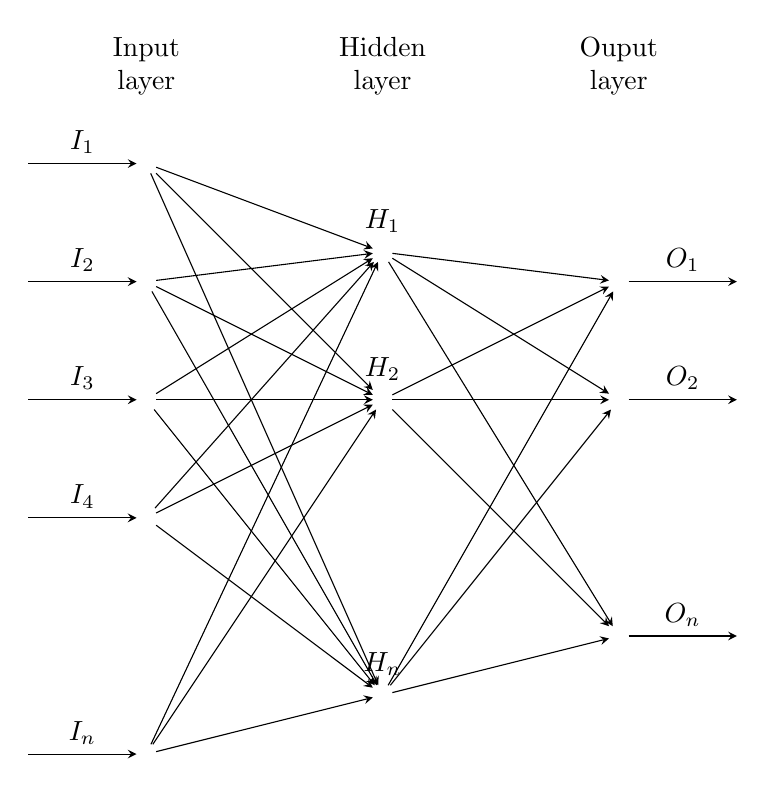
\begin{tikzpicture}[x=1.5cm, y=1.5cm, >=stealth]
					\foreach \m/\l [count=\y] in {1,2,3,4,missing,5}
  						\node [every neuron/.try, neuron \m/.try] (input-\m) at (0,2.5-\y) {};

					\foreach \m [count=\y] in {1,2,missing,3}
  						\node [every neuron/.try, neuron \m/.try ] (hidden-\m) at (2,2-\y*1.25) {};

					\foreach \m [count=\y] in {1,2,missing,3}
  						\node [every neuron/.try, neuron \m/.try ] (output-\m) at (4,1.5-\y) {};

					\foreach \l [count=\i] in {1,2,3,4,n}
  						\draw [<-] (input-\i) -- ++(-1,0)
    							node [above, midway] {$I_\l$};

					\foreach \l [count=\i] in {1,2,n}
  						\node [above] at (hidden-\i.north) {$H_\l$};

					\foreach \l [count=\i] in {1,2,n}
  						\draw [->] (output-\i) -- ++(1,0)
    							node [above, midway] {$O_\l$};

					\foreach \i in {1,...,5}
  						\foreach \j in {1,...,3}
    							\draw [->] (input-\i) -- (hidden-\j);

					\foreach \i in {1,...,3}
  						\foreach \j in {1,...,3}
    							\draw [->] (hidden-\i) -- (output-\j);

					\foreach \l [count=\x from 0] in {Input, Hidden, Ouput}
  						\node [align=center, above] at (\x*2,2) {\l \\ layer};

				\end{tikzpicture}
		\end{figure}

		\begin{HighlightedNote}{}
			However, sometimes you will need more complicated diagrams (or maybe you do not like TiKZ, in that case I recommend a vector drawing tool such as Inkscape which allows \LaTeX \,embedding)
		\end{HighlightedNote}

		\subsection{Figures} \label{sub:figures}

		\begin{HighlightedNote}{}
			In general the best way to visualize your results will be some figures, I recommend Python's matplotlib for generating them or any other tool you are familiar with.
		\end{HighlightedNote}

		% \begin{figure}[htp]
    	% 		\centering
		% 		\begin{subfigure}{0.48\textwidth}
        % 					\centering
        % 						\includegraphics[width=\textwidth]{figures/sfem_1D_p3.pdf}
        % 						\caption{One-dimensional spectral element basis functions of polynomial degree $p = 3$ for subspace $G_{3} \subset H^{1}(\Omega)$, $\Omega\in\mathbb{R}$.}
    	% 			\end{subfigure}
    	% 			\hspace{.35cm}
    	% 			\begin{subfigure}{0.48\textwidth}
        % 					\centering
        % 						\includegraphics[width=\textwidth]{figures/sfem_1D_p5.pdf}
        % 						\caption{One-dimensional spectral element basis functions of polynomial degree $p = 5$ for the subspace $G_{5} \subset H^{1}(\Omega)$, $\Omega\in\mathbb{R}$.}
    	% 			\end{subfigure}

		% 		\vspace{1cm}

		% 		\begin{subfigure}{0.48\textwidth}
        % 					\centering
        % 						\includegraphics[width=\textwidth]{figures/sfem_p3.png}
        % 						\caption{Two-dimensional spectral element basis functions of polynomial degree $p = 3$ for subspace $G_{3} \subset H^{1}(\Omega)$, $\Omega\in\mathbb{R}^{2}$.}
    	% 			\end{subfigure}
    	% 			\hspace{.35cm}
    	% 			\begin{subfigure}{0.48\textwidth}
        % 					\centering
        % 						\includegraphics[width=\textwidth]{figures/sfem_p5.png}
        % 						\caption{Two-dimensional spectral element basis functions of polynomial degree $p = 5$ for the subspace $G_{5} \subset H^{1}(\Omega)$, $\Omega\in\mathbb{R}^{2}$.}
    	% 			\end{subfigure}

   		% 		\vspace{.25cm}
    	% 			\caption{Example basis functions for the spectral finite element method in 1D and 2D.}
    	% 			\label{fig:plots}
		% \end{figure}

% subsection figures (end)

\subsection{Tables} % (fold)
\label{sub:tables}

\begin{HighlightedNote}{}
\LaTeX \; booktab environments are really good to showcase and track your results, however they can get fairly messy. My suggestion is to generate them via Python automatically and store the results in either a plain text file or a spreadsheet (there are packages to read spreadsheets with Python)
\end{HighlightedNote}

\begin{table}[ht]
     \centering
     \begin{tabular}{rrrrrrrrrr}
         $\upsigma \setminus \tau$ & \multicolumn{1}{c}{0} &\multicolumn{1}{c}{1} &\multicolumn{1}{c}{2} &\multicolumn{1}{c}{3} &\multicolumn{1}{c}{4} &\multicolumn{1}{c}{5} &\multicolumn{1}{c}{6} &\multicolumn{1}{c}{7} &\multicolumn{1}{c}{8}\\
          \midrule
         0.0 & 100.0  &100.0  &100.0  &100.0  &100.0  &100.0  &100.0  &100.0  &100.0 \\
         0.2 & 100.0  &100.0  &100.0  &100.0  &100.0  &100.0  &100.0  &100.0  &100.0 \\
         0.4 & 100.0  &100.0  &100.0  &100.0  &100.0  &100.0  &100.0  &100.0  &100.0 \\
         0.6 & 98.6  &100.0  &100.0  &100.0  &100.0  &100.0  &100.0  &100.0  &100.0 \\
         0.8 & 84.7  &99.5  &100.0  &100.0  &100.0  &100.0  &100.0  &100.0  &100.0 \\
         1.0 & 28.1  &98.3  &99.9  &100.0  &100.0  &100.0  &100.0  &100.0  &100.0 \\
         1.2 & 1.3  &88.7  &99.4  &99.9  &99.8  &99.9  &100.0  &99.9  &100.0 \\
         1.4 & 0.0  &57.1  &96.2  &99.3  &99.0  &99.3  &99.4  &99.8  &99.7 \\
         1.6 & 0.0  &18.6  &81.2  &93.0  &93.7  &94.8  &95.6  &92.3  &93.3 \\
         1.8 & 0.0  &2.4  &42.8  &67.0  &70.1  &72.1  &69.0  &69.1  &68.6 \\
         2.0 & 0.0  &0.1  &9.0  &23.1  &24.5  &26.9  &28.2  &27.3  &27.3 \\
         \midrule
          $t$(ms) &27.92 &40.23 &77.30 &157.27 &252.05 &342.18 &381.46 &399.85 &413.72\\
     \end{tabular}
     \caption{Performance of the algorithm for 128-bit key and with multiple readings per key}
     \label{tab:error_128_avg}
 \end{table}





		% \begin{figure}[h]
    	% 		\includegraphics[width=0.9\textwidth]{figures/LSTM}
    	% 		\centering
    	% 		\caption{Gate Recurrent Unit in a Long Short Term Memory Neural Netwok (GRU-LSTM). \\ \emph{Credit to \url{https://colah.github.io/posts/2015-08-Understanding-LSTMs/}}}
    	% 		\label{fig:LSTM}
		% \end{figure}


\section{Topic C to focus on} \label{sec:topic_c}
% subsection tables (end)

% section results (end)




%----------------------------------------------------------------------------------------
%   REFERENCE LIST
%----------------------------------------------------------------------------------------
\appendix

%% References (bibliography)
\section{References}
	\begin{HighlightedNote}{}
		Do not forget to cite the papers that you are using in your research, this way your work will be infinitely easier to write down and to review when the time comes.
	\end{HighlightedNote}

	% Add the bibliography without the header. You can remove the heading=none and \section{References} to have it in a different way.
	% Here we keep the references as a section from the Appendix, as an example
	\printbibliography[heading=none]


\section{Resources}
	\begin{HighlightedNote}{}
		It is a good idea to record sources that explain concepts or provide tools so the research is both better documented and if someone has to continue it there is enough supporting documentation.
	\end{HighlightedNote}
	\begin{itemize}
    		\item Quick read in DTW and Keogh Lower Bounding. \newline
			\url{http://alexminnaar.com/time-series-classification-and-clustering-with-python.html} \newline
			\url{http://nbviewer.jupyter.org/github/alexminnaar/time-series-classification-and-clustering/blob/master/Time%20Series%20Classification%20and%20Clustering.ipynb}

		\item Parallelizing DTW -- Good article on making a parallel version of DTW. Uses Keogh lower bound not as a linear approximation but as a pruning device. \newline
			\url{https://www.andrew.cmu.edu/user/mmohta/15418Project/finalreport.html}

    		\item Deep Learning
    			\begin{itemize}
        				\item Intro to LSTM \newline
					\url{https://colah.github.io/posts/2015-08-Understanding-LSTMs}
        				\item Intro to CNN \newline
					 \url{https://colah.github.io/posts/2014-07-Conv-Nets-Modular/}
				 \item Why are LSTMs are so useful, impressive result in character pattern and syntax learning \newline
					\url{https://karpathy.github.io/2015/05/21/rnn-effectiveness/}
    			\end{itemize}
	\end{itemize}


%% Add the list of todos in the end
\section{TODOS}
	\begin{HighlightedNote}{}
		Here you will have all your TODOs grouped with anchor links to the parts of the document where they are. Really handy if you do not know where to continue with your project.
	\end{HighlightedNote}

	\AddListOfTodos

\end{document}